\documentclass{article}
\usepackage{amsmath}
\usepackage{amssymb}
\usepackage{graphicx}
\usepackage{hyperref}
\usepackage[version=4]{mhchem}


\begin{document}
\section*{Problem}
In triangle \(A B C, A D\) is the median on \(B C . B G\) and \(B H\) divide \(A D\) into three parts such that \(A E: E F: F D=4: 3: 1 . A G: G H\) : \(H C=x: y: z\). Find the value of \(x+y+z\), where \(x\) and \(y\) are positive integers relatively prime.\\
\centering
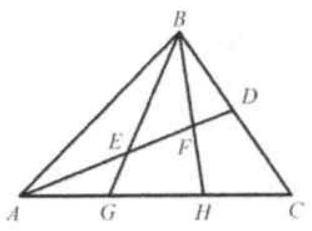
\includegraphics[width=\textwidth]{images/129(2).jpg}

\section*{Solution}
9.
Extend \(A D\) to \(M\) and \(N\) and connect \(C M\) and \(C N\) such that \(D M=D F\) and \(D N=\) \(D E\). So \(B F C M\) and \(B E C N\) are parallelograms since the diagonals bisect each other.\\
Thus \(B E / / N C, B F / / M C\).\\
\centering
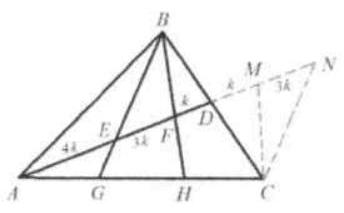
\includegraphics[width=\textwidth]{images/140(1).jpg}

Let \(A E=4 k, F E=3 k\), and \(F D=k\). So \(F M N=3 k\), and \(D M=k\).\\
Since \(B E / / N C, \triangle A G E \sim \triangle A C N . \frac{A E}{A N}=\frac{A G}{A C}=\frac{4 k}{12 k}=\frac{1}{3} \quad \Rightarrow\) \(A G=\frac{1}{3} A C=\frac{3}{9} A C\)

Since \(B H / / M C . \triangle A H F \sim \triangle A C M\).\\
\centering
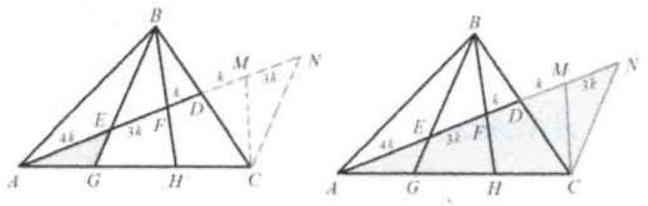
\includegraphics[width=\textwidth]{images/140(3).jpg}\\
\(\frac{A F}{A M}=\frac{A H}{A C}=\frac{7 k}{9 k}=\frac{7}{9} \Rightarrow A H=\frac{7}{9} A C\).\\
\(G H=A H-A G=\frac{7}{9} A C-\frac{3}{9} A C=\frac{4}{9} A C\).\\
\(H C=A C-A H=A C-\frac{7}{9} A C=\frac{2}{9} A C\).\\
\centering
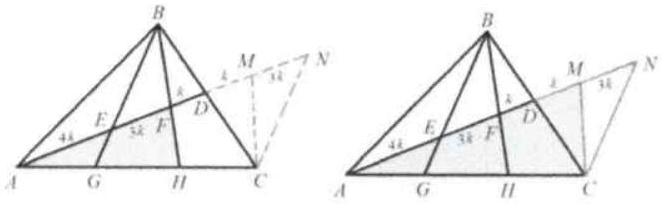
\includegraphics[width=\textwidth]{images/140.jpg}\\
\(A G: G H: H C=3: 4: 2\). The answer is \(3+4+2=9\).

\end{document}
